\documentclass{standalone}
\usepackage{tikz}
\usepackage{fkmath}
\begin{document}
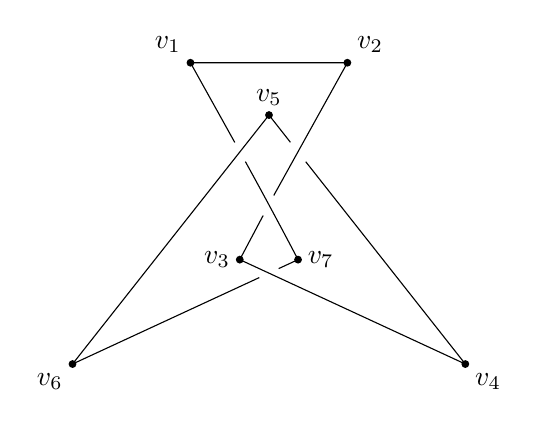
\begin{tikzpicture}
  \draw[draw=black, opacity=1, line width=0.4pt] (2.77282781998861,
  -1.0171886237063246) -- (2.500942875021245, -0.6714280399856819)
  node (v4) {} -- (2.500942875021245, -0.6714280399856819) .. controls
  (2.0842623999672862, -1.1983593364079537) and (1.6685247289402927,
  -1.7254015116953847) .. (1.2527870295155876, -2.2524438715679413) --
  (1.2527870295155876, -2.2524438715679413) .. controls
  (0.8164514049128893, -2.8055963654336806) and (0.38152322769526587,
  -3.3569669028930313) .. (0.005574020836252973, -3.8335706672084946)
  -- (0.005574020836252973, -3.8335706672084946) node (v5) {} ..
  controls (0.8464479503312664, -3.444322381613845) and
  (1.6695599675186974, -3.0632966534290733) .. (2.377671816449687,
  -2.7355047075596555);

  \draw[opacity=1, line width=0.4pt] (2.6238328363023853,
  -2.621554345907698) -- (2.6238328363023853, -2.621554345907698) ..
  controls (2.705886604245657, -2.5835711286713097) and
  (2.78794023020037, -2.545587627457804) .. (2.869993998143642,
  -2.5076042682328574) -- (2.869993998143642, -2.5076042682328574)
  node (v6) {} .. controls (2.639982756909483, -2.06851885061398) and
  (2.407155030633322, -1.6365932060462707) .. (2.2009069945125685,
  -1.2623818353469443);

  \draw[opacity=1, line width=0.4pt] (2.0662717396906722,
  -1.0188432447736497) -- (2.0662717396906722, -1.0188432447736497) ..
  controls (1.8738370604619938, -0.6717144309077286) and
  (1.6900946367939778, -0.34321639013684996) .. (1.5036735989740475,
  -0.007099440550881529) node (v0) {} -- (1.5036735989740475,
  -0.007099440550881529) .. controls (2.1678912469875353,
  -0.007099440550881529) and (2.8321087530124647,
  -0.007099412153169874) .. (3.4963264010259527,
  -0.007099440550881529) node (v1) {} -- (2.5613679518477044,
  -1.6929128256986796);

  \draw[opacity=1, line width=0.4pt] (2.4265672803554144,
  -1.9475038482449007) -- (2.4265672803554144, -1.9475038482449007) ..
  controls (2.32452407920065, -2.140228042143908) and
  (2.2179281569132594, -2.341550211200881) .. (2.1300060018563585,
  -2.507604268232857) node (v2) {} -- (4.9944259551676815,
  -3.8335708091970533) node (v3) {} -- (4.9944259551676815,
  -3.8335708091970533) .. controls (4.3243319686812995,
  -2.9840742793264234) and (3.5891526988972178, -2.052065784434959) ..
  (2.967704844408228, -1.2642397556320117);

  \foreach \n in {0,1,2,3,4,5,6}{
    \node[fill, circle, inner sep=1pt] () at (v\n) {};
  }

  \begin{scope}[every node/.style={scale=1}]
    \node[above left] () at (v0) {$\msf{v_1}$};
    \node[above right] () at (v1) {$\msf{v_2}$};
    \node[left] () at (v2) {$\msf{v_3}$};
    \node[below right] () at (v3) {$\msf{v_4}$};
    \node[above] () at (v4) {$\msf{v_5}$};
    \node[below left] () at (v5) {$\msf{v_6}$};
    \node[right] () at (v6) {$\msf{v_7}$};
  \end{scope}
\end{tikzpicture}
\end{document}
